\chapter{Estimating panel angles}
Solar panel installation angles are a large factor in deciding the energy output of a PV system. If panel angles can be freely chosen during planning and installation phases, it can make sense to either optimize for total power generation or power generation during peak consumption hours. This means that even if installation angles could be freely chosen, installation angles are unlikely to be the same for every system in the same geographical region. Panel angles may also be restricted by installation sites and mounting types.

% Panel racks have to be installed based on the available area 

%Installation type also plays a factor in choosing the panel angles. Panel angles may be restricted by 

 %In so called flush rooftop installations, the panels are installed to run along the roof and so the angles can not be freely chosen. Panels can also be rack mounted and these racks tend to be installed and oriented based on the available area as is the case with \ref{fig_fmikumpula_panels}. Due to the forementioned reasons, panel angles vary from installation to installation.

One reason for lacking of faulty metadata is that panel angles can be difficult to measure accurately. The tilt angle of the panels or the angle between the panel normal and zenith(the point directly above) can easily be measured with an angle ruler and a bubble level, but the azimuth angle of the panels is much harder to measure with the same degree of accuracy. If an accurate compass is used and the difference between the magnetic north and the geographic north is taken into account, metal structures and electrical systems nearby can still distort local magnetic fields enough to cause errors in measurements. The challenges in taking accurate measurements are not insurmountable, but they may contribute to the inaccuracies and the lack of available information in PV installation parameter metadata. 

The space of possible panel installation angles can be thought as a half unit sphere in a spherical coordinate system where each point on the surface represents a direction to which the normal of the solar panels could be directed towards. A visualization of parameter space in 3D and 2D is shown in \ref{fig_halfdome} and \ref{fig_anglespace1}. The 3 dots in the subfigure \ref{fig_anglespace1} mark the zenit for which azimuth is not well defined(red), the installation angles of FMI Helsinki installation azimuth $135^\circ$ tilt $15^\circ$(blue) and a close to power generation maximized installation with directly south facing panels with the tilt of $45^\circ$(black).


\begin{figure}[h]
	
     \centering
     \begin{subfigure}[b]{0.35\textwidth}
         \centering
         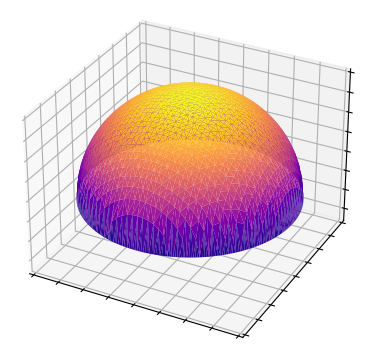
\includegraphics[width=\textwidth]{pics/halfdome}
         \caption{The space of possible angles as a 3D half sphere surface. Each point represents a possible tilt and azimuth combination.}
         \label{fig_halfdome}
     \end{subfigure}
     \hfill
     \begin{subfigure}[b]{0.35\textwidth}
         \centering
         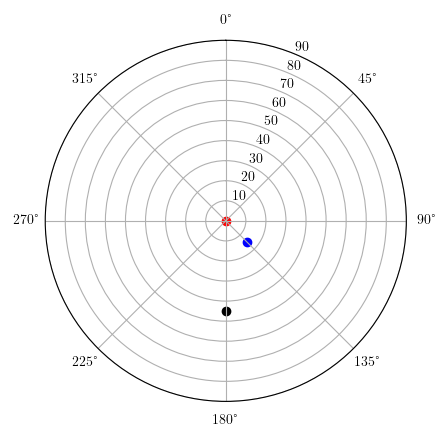
\includegraphics[width=\textwidth]{pics/polarplot}
         \caption{2D projection of the angle space, distance from center denotes the tilt angle of the panels and angle marks the azimuth.}
         
         \label{fig_anglespace1}
     \end{subfigure}
     \hfill
     \caption{Angle space visualizations.}
     \label{fig_anglespace}
\end{figure}


\noindent Estimating panel installation angles requires the use of multiple functions, each of which can be defined in multiple ways. These functions are defined in the following sections.
\begin{itemize}
  \item Prediction error function for quantifying how good a prediction was when the correct panel parameters are known.
  \item Model fitness function for measuring the difference between simulated power values and measured power values.
  %\item Multiplier matching function for matching the magnitude of simulated power values with the magnitude of measurements.
  \item Angle space discretization function for discretizing the angle space into $n$ discrete points which can then be tested with model fitness function.
\end{itemize}




\section{Prediction error function}
%The first part in developing a panel installation estimation algorithm is creating a metric for measuring how well the algorithm performs. 
In this thesis, the proposed error estimation method combines the tilt and azimuth delta values into one error angle value, the angular distance between two points on a spherical surface. The goal is then to develop a panel angle estimation function which achieves the lowest angle error value with the available datasets.

Alternative approaches can also be chosen as the function or functions for measuring the distance between two points in angle space can be defined in multiple ways. The simplest way is to use the delta of known tilt and azimuth angles as two separate error values without normalizing in any way. This method was used in Hagdadi's 2017\cite{navid_australian_article} article but such values are not direcly comparable between installations as the significance of azimuth delta depends on tilt angle.

%Measuring the distance between two coordinate pairs in angle space is more complicated than measuring errors in latitudinal or longitudinal degrees. This difficulty rises from how the azimuth angle lines converge at the pole, resulting in a coordinate system where azimuth delta values are disconnected from the phenomena which they are trying to describe. If the tilt angle is near zero, azimuth delta becomes meaningless but at high tilt angles, even small azimuth delta values can be significant. If this is not corrected for, using azimuth and tilt deltas (changes in angles) as algorithm performance metrics would incorrectly suggest that the data quality of low tilt installations is lower than that of high tilt installations, or that the system is less capable of estimating the parameters of low tilt installations. Due to these reasons, a better way of measuring the distance between two points is needed, luckily the center angle between two points on an unit sphere is easy to solve with geometry and the resulting equation is rather simple.

%While there are no issues with using angles to denote the direction of the panels, the angle values do not map the possible panel angles into the angle space in a way which would make measuring the difference between two angle space coordinates easy. The issues rises from how the azimuth angle lines converge at the pole, resulting in a coordinate system where azimuth delta values are disconnected from the phenomena which they are trying to describe. For example, a 45 degree azimuth delta is fairly significant at tilt of 90 degrees but almost insignificant at 15 degree tilt. If this is not corrected for, using azimuth and tilt deltas (changes in angles) as algorithm performance metrics would incorrectly suggest that the data quality of low tilt installations is lower than that of high tilt installations, or that the system is less capable of estimating the parameters of low tilt installations. Due to these reasons, a better way of measuring the distance between two points is needed, luckily the center angle between two points on an unit sphere is easy to solve with some geometry and the resulting equation is rather simple.

\vspace{3mm}
\noindent\textbf{Deriving angle space distance equation}

\noindent Let $v= [v_1, v_2]$ and $k = [k_1, k_2]$ be two component angle-space vectors so that $v_1$, $k_1$ $\in$ $[0,90]$ and $v_2$, $k_2$ $\in [0,360]$. These vectors represent points on the surface of a unit sphere and their components are the angles of spherical coordinate system. The cartesian coordinates of these points are:
	\begin{align}
	x_v &= sin(v_1)cos(v_2)\\
	y_v &= sin(v_1)sin(v_2)\\
	z_v &= cos(v_1)
  \end{align}
  And
  \begin{align}
	x_k &= sin(v_1)cos(v_2)\\
	y_k &= sin(v_1)sin(v_2)\\
	z_k &= cos(v_1)
  \end{align}
\noindent And the cartesian distance between these two points can be calculated with the following equation:
\begin{align}
	d = \sqrt{(x_v-x_k)^2 + (y_v-y_k)^2+(z_v-z_k)^2}
\end{align}


\noindent The two points and the origin form an isoceles triangle with the sides from the origin to the vector end points having the length of 1 while the distance between the vector end points is the same as d.

\noindent As the lengths of three sides are known, the angles of the triangle can be calculated with the cosine rule. 
\begin{align}
	a^2 &= b^2 + c^2 - 2bc \cos(A)
\end{align}
Where
\begin{conditions}
 a     &  Side opposing the angle A, same as earlier value d \\
 b     &  Side opposing angle B, value is 1  \\   
 c	   &  Side opposing angle C, value is 1
\end{conditions}
\noindent Substituting known values into the cosine equation.

\begin{align}
	a^2 &= b^2 + c^2 - 2bc \cos(A)\\
	d^2 &= 1^2 + 1^2 - 2 \cos(A) \\
	d^2 &= 2 - 2 \cos(A)
\end{align}

\noindent Solving for angle A
\begin{align}
	d^2 &= 2-2\cos(A)\\
	2 \cos(A) &= 2 -d^2 \\
	\cos(A) &= \frac{2-d^2}{2} \\
	A &= \cos^{-1}(\frac{2-d^2}{2})
\end{align}

\noindent Renaming $A$ as $Error$.

\begin{align}
	Error &= \cos^{-1}(\frac{2-d^2}{2}) \label{errorangle}
\end{align}


\noindent By first calculating the distance between the vectors using equations 5.1-5.7 and then substituting the distance into equation 5.16, the resulting angle can then be used as an error value between two panel angle measurements. Python code based on this proof is included in appedix \ref{angular_distace_appendix}.


% This error value is the same as the angle between two points on the surface of a sphere. %In addition, if the deviation occurs only on the tilt axis, the error value and the tilt error are the same.% This makes the error values intuitive.
%In some ways, this method of calculating an error angle is analogous to moving the two angle vectors so that one of them aligns with the 0 tilt point and computing the tilt delta between the two points. Because of this, the error values are fairly intuitive and the error value should better represent the actual difference between installations than other error values calculated via other means.


\vspace{5mm}

%\section{Angle estimation error functions}
%The process of angle estimation requires the use of error estimation functions. The first function is needed for testing the accuracy of the algorithm by translating the known installation angles and the estimated angles into a meaningful error value. This is nontrivial as moving by a set angle value on the tilt and azimuth axis in spherical coordinate space result in different cartesian distances depending on the starting point. 


%The second function or set of functions is needed for evaluating how well a simulated irradiance curve fits the measurement data. Functions of this type can be used for parameter estimation by testing out possible parameter combinations and and choosing the combination which results in the lowest error between the simulated and measured values.


\newpage
\section{Simulation fitness function}
\label{section_simulation_error_function}

The earlier model error function defined in \ref{pv_model_delta} can be re-used as the simulation fitness function. By then computing multiple simulations with different panel angles and choosing the simulation with the best fitness, meaning lowest delta value, the panel angle values can be estimated.

\vspace{6mm}
\noindent\textbf{Simulation fitness function}
\begin{equation}
\begin{split}
\label{pv_model_delta}
Delta_{model} = \sum_{t=1}^{1440} |P_{measured}(t) - P_{simulated}(t)| /1440
\end{split}
\end{equation}

\noindent As the function normalizes delta values by division with 1440, the delta for shorter days is lower than the delta for comparable long days. This should not matter for parameter estimation as the algorithm works by minimizing delta for each day independently. 

Visualization of the function is shown in \ref{fig_simulation_fitness} where simulation with tilt of 90 degrees and azimuth of 135 is tested against known power measurements from a day in FMI Helsinki dataset, resulting in an average delta of 2959.5 W delta per minute.



\begin{figure}[h]
\centering
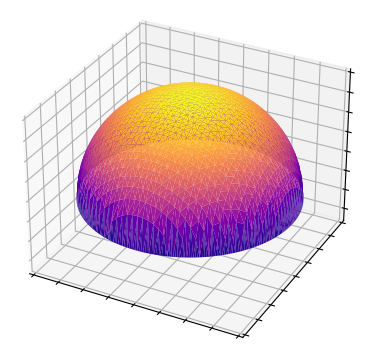
\includegraphics[width=0.8\linewidth]{pics/halfdome} % WAS pics/measured_vs_simulated
\figcaption{Visualization of fitness function.}
\label{fig_simulation_fitness}
\end{figure}




%The earlier simulation error function defined in \ref{pv_model_delta} can be used for evaluating how well a simulated power output curve fits measured power data. By then simulating the power output with several installation parameters and 


%By simulating power generation with different parameter combinations and choosing the set of parameters with the lowest delta value, 



%Simulation error function measures how much the predicted power generation values vary from the measured power generation values. The purpose of the simulation error function is to be able to generate a single numerical value which describes how well a certain parameter combination models the measurements. By then testing out multiple parameter combinations, the combination with the lowest simulation error function value should be the best fit and the parameters used for the simulation should be within a small error of the physical parameters of the solar PV installation. In \ref{fig_error} the error between a cloud free day and randomly chosen set of wrong simulation parameters is visualized.


\newpage
\section{Angle space discretization}\label{angle_space_discretization}
The next step is angle space discretization. The panel angles are denoted with a doublet of tilt and azimuth values, ranging from 0 to 90 and 0 to 360 respectively. If the tilt and azimuth axes are discretized individually in steps of 5 so that tilt is [0, 5, 10, 15... 90] and azimuth [0, 5, 10, 15... 355], the permuations of these tilt and azimuth values create an even grid in the euclidean projection of angle space where x = tilt, y = azimuth. However as the physical phenomena represented by the angle values is not a point on a flat plane but a point on a half-sphere surface, this results in an uneven discretization seen in figure \ref{fig_5step}. 

Sphere discretization problems are relevant for 3D graphics and real world problems involving geometry and so there are pre-existing methods available for discretization. One of the mathematically more elegant methods is the Fibonacci lattice which was used in a similar fashion in González 2009 \cite{Gonzlez}. The mathematical formulation of similar lattices is an older process and an earlier example is found in Vogel 1979\cite{fibolat_old}. The following mathematical notation for the lattice is based on a code sample included in a blog post by Vagner Seibert \cite{medium_fibolat_equation}.




\noindent \textbf{Fibonacci lattice point n of k equation}
\begin{align}
	s &= n + 0.5 \\
	\phi &= acos(1 - 2 s / k) \\
	\theta &= \pi s (1 + \sqrt{5})
\end{align}
Where $n$ is the point number, $k$ is the amount of points, $\phi$ is the panel tilt angle and $\theta$ is the azimuth angle.
\begin{align}
	x &= cos(\theta)sin(\phi)\\
	y &= sin(\theta)sin(\phi)\\
	z &= cos(\phi)
\end{align}
$x$, $y$ and $z$ are the corresponding cartesian coordinates.
\vspace{5mm}


\begin{figure}
     \centering
     \begin{subfigure}[b]{0.45\textwidth}
         \centering
         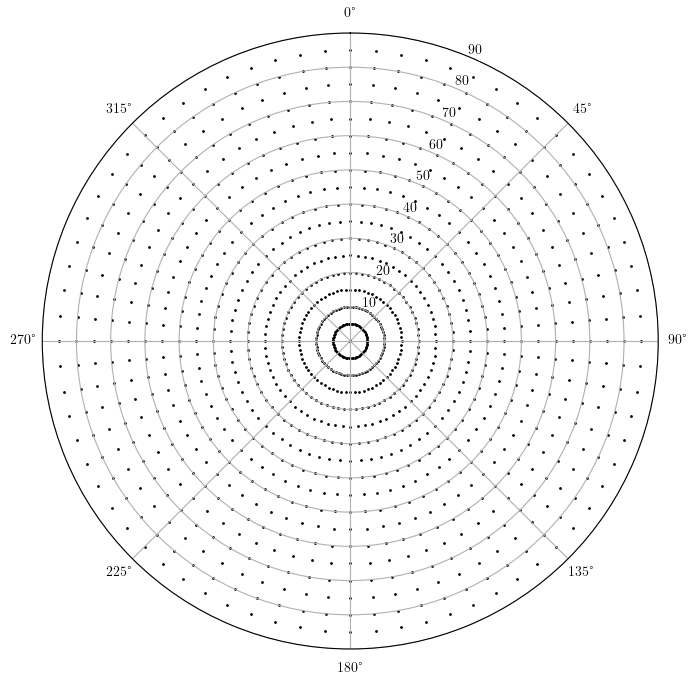
\includegraphics[width=\textwidth]{pics/disc5}
         \caption{In steps of 5 discretization with 1296 points}
         \label{fig_5step}
     \end{subfigure}
     \hfill
     \begin{subfigure}[b]{0.45\textwidth}
         \centering
         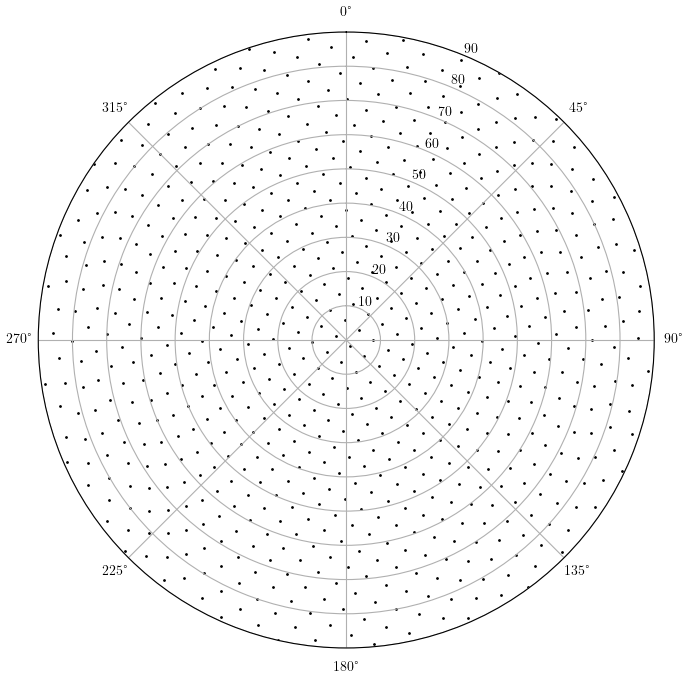
\includegraphics[width=\textwidth]{pics/fibolat1}
         \caption{Fibonacci lattice-based discretization with 756 points.}
         \label{fig_fibolat}
     \end{subfigure}
     \hfill
     
\caption{Comparison of two different discretization patterns. Fibonacci lattice based discretization on right shows a more even distribution of points than the latitude-longitude lattice. The minimum density is approximately the same in both graphs despite the difference in point counts.}
     \label{fig_5stepfibolat}
\end{figure}

\newpage
\subsection{Importance of lattice density}\label{ss_lattice_density}
Using the correct lattice density is important for using exhaustive search algorithms for panel angle estimation. Regardless of the lattice point count, a discrete lattice is unlikely to ever include the best fit in the whole $\mathbb{R}^2$ parameter subspace. This means that if the lattice density is low, distance between best fit and closest lattice points can result in significant errors. However as incresing the lattice density increases the computational cost of angle estimation, choosing a good density is an optimization problem.

With \textit{in-steps-of-n} lattices, the main benefit is easy readibility. If the lattice is given one point for latitudinal and longitudinal degree, resulting in $360*90=32400$ points, then the lattice can be aligned so that each tilt and azimuth degree pair where angles are integers is tested. This discretization makes the results easily understanble as if the known installation angles are given as integers, a point representing the exact known installation angles already exists on the lattice. The same applies for lower density in \textit{in-steps-of-n} lattices.

If a Fibonacci lattice or some other discretization method is used, evaluating the performance of the fitting algorithm is not as easy. With an $n$ point Fibonacci lattice the distance between lattice points varies slightly and and it may be difficult to estimate where the closest points to the known installation angles are.




%The density of lattices is an important measurable charasteristic which proves useful during the optimization of angle estimation algorithm. The most useful metric would be the sphere center angle distance between neighboring points. This would be useful as it can be used for determining whether errors in predictions are lattice or function fitting related. For example, if the lattice neighbors are approximately 1 degree away from oneanother and the predicted angle is 5 degrees off from the known installation angle, then the error is caused by model fitting and not lattice density as there must have been multiple lattice points closer to the known angle point than the discovered best fit. However if grid density is near to or lower than angle estimation error, the lattice is likely to be a contriburing to angle estimation errors.

%Calculating neighborign center angle distances for both \textit{in-steps-of-n} and Fibonacci lattices is somewhat challenging. In \textit{in-steps-of-n}, the value \textit{n} can be used as an estimate for max center angle distance as \textit{n} will always be the tilt distance to the nearest neighbor with different tilt angle. With Fibonacci lattices the easiest way of estimating center angle distances is taking the coordinates of the first two lattice points and calculating their center angle distance with earlier error equation \ref{errorangle}. These first two points should be used as Fibonacci lattice points are distributed on a single arm spiral pattern, resulting in later sequential points being further from one another.

%Another method for calculating Fibonacci lattice point distances is dividing the surface area of the angle space by the amount of calculated lattice points. This area-per-point value could then be used in order to estimate how far points are from oneanother on average. In later sections, the first two points derived distance will be used.

\newpage
\section{Solving panel angles}
Now that the geographic location and multiplier value of installation are known to be solvable and fitness functions have been defined, the next step is solving the panel angles. The simple method is evaluating all points on a sufficiently dense lattice and choosing the point with the lowest delta value.

Figure \ref{fig_polar10} contains 10 fibonacci lattice points and their normalized delta values. The best fit was at tilt 31.79$^\circ$, azimuth 153.79$^\circ$ and delta value of 369W. The lattice density leaves large gaps between lattice points and this found best fit is the closest point to the known installation angles of 15$^\circ$ and 135$^\circ$. Center angle error as per \ref{errorangle} is 18.17$^\circ$.




%is to solve the panel installation angles. The chosen method relies on splitting angle space into $n$ discrete points and evaluatin each of their fitness by calculating an error value. Here the angle space was split into 10 discrete points with fibonacci lattice \ref{angle_space_discretization} and the fitness of each point was evaluated with area error \ref{areaerror} and multiplier matching \ref{function_multipliermatch} functions. %The tilt-azimuth pair with the lowest error value was 31 


\begin{figure}[h]
\begin{floatrow}
\ffigbox{%
  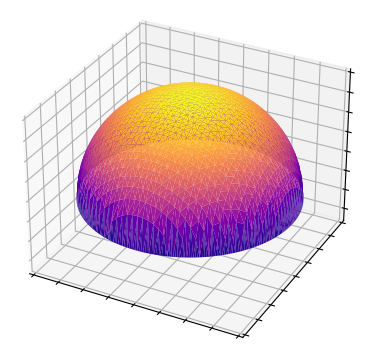
\includegraphics[width=1\linewidth]{pics/halfdome} % WAS pics/10p_fibo_fit_text
}{
  \caption{Polar plot of test points for a single day of data from FMI Kumpula dataset.}
  \label{fig_polar10}
}
\capbtabbox{%
  \begin{tabular}{c|c|c} \hline

Tilt$^\circ$ & Azimuth$^\circ$ & Delta(W)\\
\hline
18.19 & 291.25 & 3128\\
\textbf{31.79} & \textbf{153.74} & \textbf{369}\\
41.41 & 16.23 & 3873\\
49.46 & 238.72 & 4183\\
56.63 & 101.22 & 3356\\
63.26 & 323.71 & 6888\\
69.51 & 186.2 & 1759\\
75.52 & 48.69 & 5814\\
81.37 & 271.18 &  6626\\
87.13 & 133.68 & 2938\\
\hline\hline
\end{tabular}
}{%
  \caption{Tilt, azimuth and error table for single day.}
}
\end{floatrow}
\end{figure}

The fit achieved in \ref{fig_polar10} is not very good and better results can be achieved by increasing the lattice density. The trivial method is to use a fibonnacci lattice with a higher point count, for example the fit achieved with a 10 000 point lattice \ref{10k_fits_new_helsinki} found the best fit at tilt 14.79$^\circ$, azimuth 136.2$^\circ$ , delta value of 136.2W and center angle error of 0.3659 degrees$^\circ$. This is a much better fit but increasing the lattice density comes with a higher computational cost. Depending on code optimizations, evaluating a single day from the dataset against a 10 000 point lattice can from a minute up to several hours.

\begin{figure}[h]
\centering
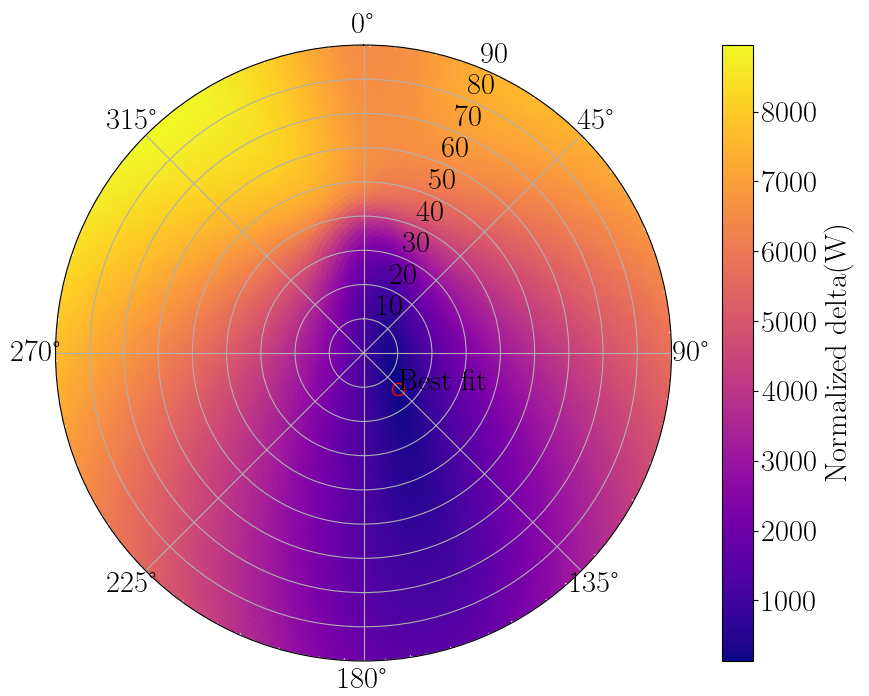
\includegraphics[width=0.8\linewidth]{pics/10k_new_model} % WAS pics/measured_vs_simulated
\figcaption{Results of a 10 000 datapoint lattice fitting against a single day from FMI Helsinki dataset. Center angle error between the found best fit and known installation angles is 0.3659 degrees$^\circ$.}
\label{10k_fits_new_helsinki}
\end{figure}



%# Best fit was tilt: 14.79 azimuth: 136.2 fitness:133.3 10k lattice result !






%\noindent Now that the method can be seen to work, it is time to improve the results. This can be done by generating larger lattices and thus by evaluating higher amount of datapoints, the algorithm has a higher chance of finding the global minimum error point. As per \ref{ss_lattice_density}, Fibonacci lattice of 1000 points would have the angular resolution of approximately 4 degrees where as 10000 points would be near to 1.5 degrees. The performance can also be improved by evaluating best fits for multiple days at once. The resulting point cloud of best fits can then be used for averaging out noise in the predictions.

%The plot \ref{fig_polar_multiyear} is a result of using the angle finding algorithm on 41 days from FMI Kumpula dataset with a Fibonacci lattice of 1000 points. The two darker spots near the center of the graph are the two most common best fits, [17.0$^\circ$, 138.4$^\circ$] with 17 and [22.7$^\circ$, 143.1$^\circ$] with 16 out of 41 days. These groupings are as close to the known installation angles of [15$^\circ$,  135$^\circ$] as could be expected from a 1000 point lattice. The next step is tightening the cluster, this can be done by adjusting the smoothness requirement of the cloud free day algorithm or by restricting the day range. In \ref{fig_polar_multiyear_summer} the tightening was accomplished with day range restrictions and 22 days were accepted by the algorithm.


%In \ref{fig_polarplot_13days} the polar plot is a result of taking the 13 best days from FMI Kumpula dataset year 2018 and using a fibonacci lattice with 500 test points. The most common best fit was [27.5$^\circ$, 150.8$^\circ$] with 5 occurances followed by [24.1$^\circ$, 138.4$^\circ$] with 4 days. These values are close to the 





%As all of the estimates converge on two neighboring points, the final step is increasing the lattice resolution further. With 10 000 point lattice, the cluster tightened further \ref{fig_polar_multiyear_helsinki10k}. Out of the 22 days, 7/22 or 32\% had best fit at [19.34, 136.87] with error of 4.38 degrees and 6/22 or 27\% at [17.74, 135.06] with error of 2.74 degrees. Rest of the best fits were distributed in smaller clusters near these points. The lowest angle distance best fit was [17.09, 130.32] with angle distance of 2.46 degrees. As the angle distance errors are higher than the discretization resolution and as the predicted angles are systematically biased, it would seem that the error is caused by the solar irradiance model or model fitting and not angle space discretization.


%As the angle distance errors are higher than the discretization resolution and as the results seem biased, the errors of the estimation algorithm would seem to be caused by inaccuracies in model fitting and not angle space discretization.




%\begin{figure}[h]
%\centering
%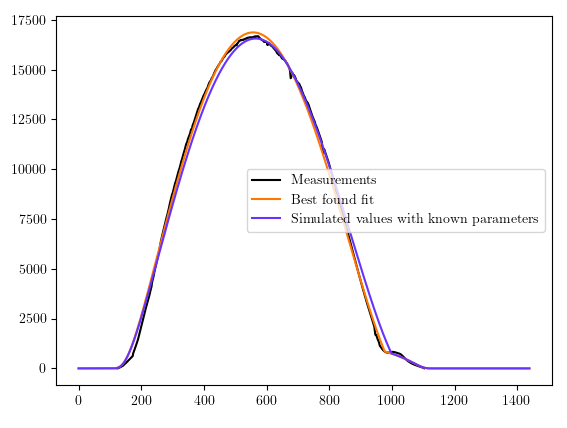
\includegraphics[width=0.8\linewidth]{pics/10kfitshelsinkiplot}
%\caption{Comparison between measured values, simulated values with known installation parameters and best found fit.}
%\label{fig_10kfitshelsinkiplot}
%\end{figure}



%day 141 predicted 17.74 135.06 delta degrees: 2.74 x
%day 145 predicted 19.92 141.6 delta degrees: 5.3
%day 148 predicted 19.34 136.87 delta degrees: 4.38 	x
%day 179 predicted 17.74 135.06 delta degrees: 2.74 x
%day 197 predicted 21.37 143.41 delta degrees: 6.87 y
%day 198 predicted 18.37 139.79 delta degrees: 3.64
%day 199 predicted 19.34 136.87 delta degrees: 4.38		x
%day 157 predicted 19.92 141.6 delta degrees: 5.3
%day 169 predicted 18.37 139.79 delta degrees: 3.64
%day 202 predicted 17.74 135.06 delta degrees: 2.74 x
%day 208 predicted 21.37 143.41 delta degrees: 6.87 y
%day 143 predicted 19.34 136.87 delta degrees: 4.38		x
%day 155 predicted 19.92 141.6 delta degrees: 5.3
%day 164 predicted 19.92 141.6 delta degrees: 5.3
%day 166 predicted 17.74 135.06 delta degrees: 2.74 x
%day 171 predicted 19.34 136.87 delta degrees: 4.38		x
%day 174 predicted 17.09 130.32 delta degrees: 2.46
%day 175 predicted 17.74 135.06 delta degrees: 2.74 x
%day 177 predicted 17.74 135.06 delta degrees: 2.74 x
%day 178 predicted 19.34 136.87 delta degrees: 4.38		x
%day 179 predicted 19.34 136.87 delta degrees: 4.38		x
%day 200 predicted 19.34 136.87 delta degrees: 4.38		x



%day 145 predicted 32.09 196.89 delta degrees: 18.65 x
%day 192 predicted 30.5 198.01 delta degrees: 16.96 y
%day 199 predicted 30.5 198.01 delta degrees: 16.96 y
%day 210 predicted 34.52 197.58 delta degrees: 20.9 z
%day 212 predicted 32.09 196.89 delta degrees: 18.65 x
%day 213 predicted 35.07 194.65 delta degrees: 21.86 k
%day 167 predicted 27.07 200.24 delta degrees: 13.37 i
%day 143 predicted 30.5 198.01 delta degrees: 16.96 y
%day 144 predicted 28.83 199.13 delta degrees: 15.21 l
%day 145 predicted 28.83 199.13 delta degrees: 15.21 l
%day 162 predicted 27.07 200.24 delta degrees: 13.37 i 
%day 167 predicted 27.07 200.24 delta degrees: 13.37 i 


\newpage
\subsection{Evaluation of exhaustive search results}
The estimated installation angles installations are fairly good. A delta of less than $4.5^\circ$ as was achieved with FMI Kumpula is small enough to be a result of measurement or rounding error. The estimates for FMI Kuopio are off by more than 10 degrees which is less encouraging. As the reported angles for FMI Kuopio were $15^\circ$ and $217^\circ$, it would seem like the angle measurements were rounded to nearest degree. This would eliminate the reporting accuracy as a plausible cause for the estimation errors and thus either there has been a reporting error or that the installation angle estimation algorithms are not performing as well for FMI Kuopio dataset.


\begin{figure}[h]
\begin{floatrow}
\capbtabbox{%
  \begin{tabular}{r|c|c|c} \hline
\multicolumn{4}{c}{FMI Kumpula}\\
\hline
n & Tilt & Azimuth & Error\\
\hline
7 & $19.34^\circ$ & $136.87^\circ$ & $4.38^\circ$\\
6 & $17.74^\circ$ & $135.06^\circ$ & $2.74^\circ$\\
4 & $19.92^\circ$ & $141.60^\circ$ & $5.30^\circ$\\
2 & $21.37^\circ$ & $143.41^\circ$ & $6.87^\circ$\\
1 & $21.37^\circ$ & $143.41^\circ$ & $6.87^\circ$\\
1 & $17.09^\circ$ & $130.32^\circ$ & $2.46^\circ$\\

\hline\hline
\end{tabular}
}{%
  \caption{Estimation results table for FMI Kumpula.}
}
\capbtabbox{%
  \begin{tabular}{c|c|c|c} \hline
\multicolumn{4}{c}{FMI Kuopio}\\
\hline
n & Tilt & Azimuth & Error\\
\hline
3 & $27.07^\circ$ & $200.24^\circ$ & $13.37^\circ$\\
3 & $30.50^\circ$ & $198.01^\circ$ & $16.96^\circ$\\
2 & $28.83^\circ$ & $199.13^\circ$ & $15.21^\circ$\\
2 & $32.09^\circ$ & $196.89^\circ$ & $18.65^\circ$\\
1 & $34.52^\circ$ & $197.58^\circ$ & $20.90^\circ$\\
1 & $34.52^\circ$ & $197.58^\circ$ & $20.90^\circ$\\
1 & $35.07^\circ$ & $194.65^\circ$ & $21.86^\circ$\\


\hline\hline
\end{tabular}
}{%
  \caption{Estimation results table for FMI Kuopio.}
}
\end{floatrow}
\end{figure}


Figures \ref{10khelsinkiplot} and \ref{10kkuopioplot} shows that the models based on best found fits are better fits than simulations done with the known parameters. This is true for both Helsinki and Kuopio datasets. This would suggest that the model fitting works as intended and that either the model is inaccurate or there is an error in reported panel angles. The more likely cause of the two is the the solar irradiance model and for some undetermined reason the error of the model is more significant for the Kuopio installation. Possible causes could be related to lower sun angles resulting in higher reflective losses or shadowing during last production hours which would also explain the uneven structure visible in the last non-zero hours in \ref{10kkuopioplot}.



\begin{figure}[h]
\caption{Comparison between a single day of measurements and two simulations. One with known installation angles and one with best found fit. Day is from FMI Kumpula dataset with reported installation angles of $15^\circ$ and $135^\circ$ degrees. Best fit at $19.34^\circ$, $136.87^\circ$}
\centering
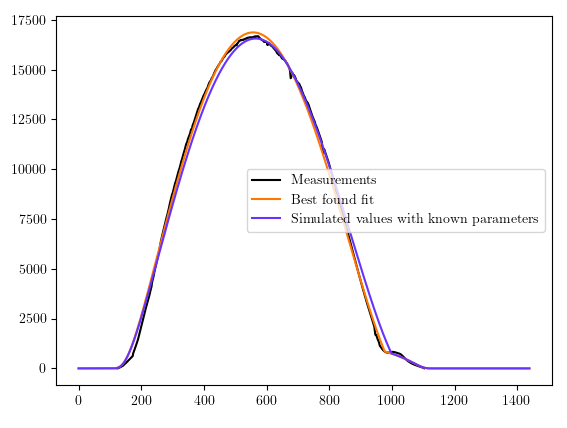
\includegraphics[width=0.6\textwidth]{pics/10kfitshelsinkiplot}
\label{10khelsinkiplot}
\end{figure}


\begin{figure}[h]
\caption{Comparison for FMI Kuopio installation. Panel angles are $15^\circ$ and $217^\circ$ degrees. Best found fit at $19.34^\circ$, $136.87^\circ$
}
\centering
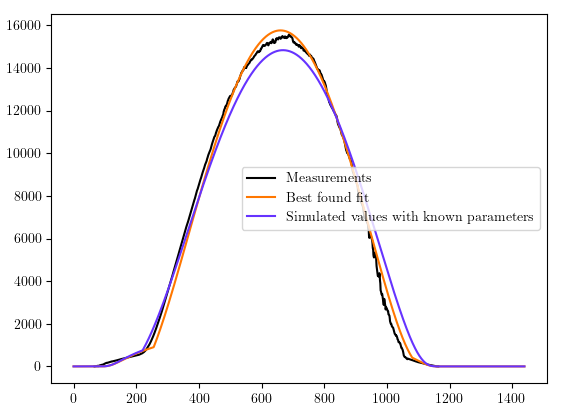
\includegraphics[width=0.6\textwidth]{pics/10kfitskuopioplots}
\label{10kkuopioplot}
\end{figure}


\section{Fast panel angle solving}
Solving panel angles by exhaustively testing 10 000 possible grid points takes up to an hour of computation time on the test system. This is not a limiting factor in research code, but exhaustive searches are inelegant compared to more intelligent approaches. Geometric intuition would suggest that the surface created by panel angle pairs and fitness values would resemble a downwards pointing cone-like shape where the best fit is the peak of the cone. If this is true, searching the whole angle space is not necessary as a gradient descent algorithm can be used to approximate the direction in which the best fit resides.

Whether the cone assumption is true can be visually examined by plotting the fitness values and observing the resulting heatmap. In \ref{fig_cone_shape}, the region where the global best fit resides is clearly the global minimum, but there appears to be a local minimum in the top part of the plot, near tilt $90^\circ$, azimuth $20^\circ$. Having more than one local minimum complicates efficient optimization but optimization is still feasible.


\begin{figure}[h]
\centering
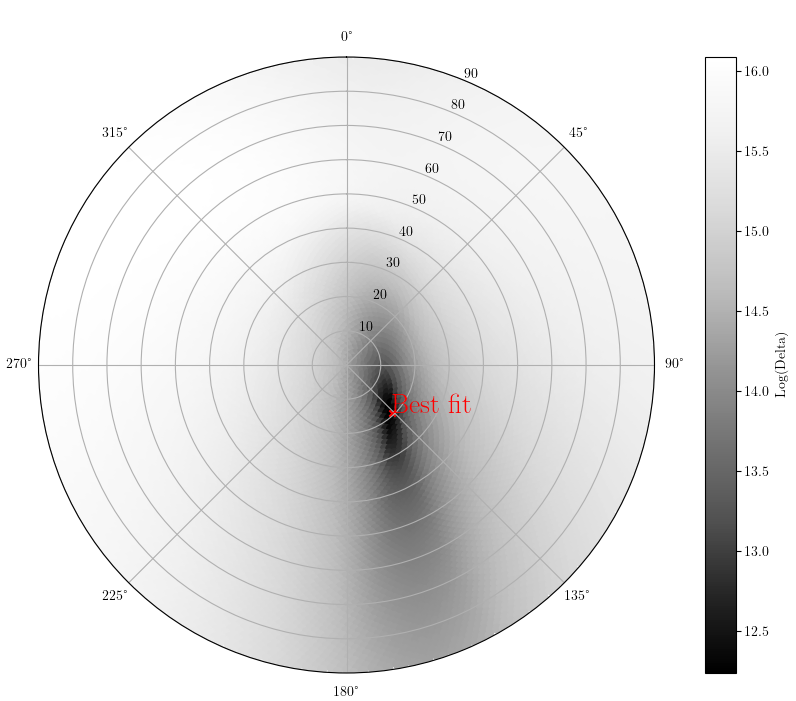
\includegraphics[width=0.6\linewidth]{pics/10kfitshelsinki}
\figcaption{Fitness heatmap.}
\label{fig_cone_shape}
\end{figure}

\subsection{Gradient search}
As the fitness surface is not defined by an easy to derivate multi parameter equation, directly solving for points where gradient reaches zero is challenging. However the gradient at a given point can still be numerically estimated and by taking steps in the direction of the gradient vector, local minimum can be found.

In x-y coordinate space, the numerical gradient for point 

\begin{align}
	\frac{\partial f}{\partial x}  &= f(p_1+x) - f(p_1)\\
	\frac{\partial f}{\partial y}  &= f(p_1+y) - f(p_1) \\
	\nabla f &= \begin{bmatrix}
	\frac{\frac{\partial f}{\partial x}}{\frac{\partial f}{\partial y}}
	\end{bmatrix} 
\end{align}

% \frac{\partial f}{\partial x} \end{bmatrix} 

% \nabla f &= \begin{bmatrix} \frac{\partial f}{\partial x \frac{\partial f}{\partial y}\end{bmatrix} 


\newpage
\subsection{Possible issues and further development ideas}

%Graphs \ref{fig_polar_multiyear_helsinki10kplot} and \ref{fig_polar_multiyear_kuopio10kplot} show that the found best fits are better fits for the data than simulations done with correct parameters. This would suggest that the model fitting and discretization both work as intended, but that the model being fitted does not work as intended. In general, the shape of the model becomes sharper when the panel tilt is near optimal in respect to sun elevation and broader when tilt deviates. This sharpening or broadening bears some reseblense to the error caused by not taking panel reflections into account and this could explain why predicted tilt angles are higher than reported installation angles. Developing a correction algorithm may be feasible, but replacing the plane of array irradiance model with a physically accurate solar power generation model is a better option.

%As the method shown earlier relies on model fitting, the accuracy of the model influences prediction accuracy. In general, the shape of the model becomes sharper when the panel tilt is near optimal in respect to sun elevation and broader when tilt deviates. This sharpening or broadening bears some reseblense to the error caused by not taking panel reflections into account and this could explain why predicted tilt angles are higher than reported installation angles. Developing a correction algorithm may be feasible, but replacing the plane of array irradiance model with a physically accurate solar power generation model is a better option.


The algorithm steps of cloud free day detection and lattice generation are computationally fast but evaluating a high density lattice for multiple days can take several minutes. For example, the time required for the generation of \ref{fig_polar_multiyear_summer} consist of 9 seconds of data loading and preprocessing, 1 second of cloud free day detection and 11 minutes of angle pair evaluation. With 22 days and 1000 points per day, the resulting 22 000 evaluations were done at the average speed of 33 evaluations per second. This comparably long processing time is due to inefficient code but the algorithms speed can also be improved by more intelligent latticing. The general location of the best fit could be solved with a low density lattice and a local high density lattice could then be used to estimate a higher accuracy angle pair. Combining code optimizations and localized angle space lattices could reduce the computation time significantly.





















